\section{Containers}

The Standard Template Library supplies the following container 
implementations:
\begin{description}
  \item[vector -- ] a random access container based on an automatically
                    resizing array.
  \item[list -- ] a random access container based on a doubly-linked
                  circular list implementation.                    
  \item[hashset -- ] a sorted collection guaranteeing that each element is
                 only contained once. It is typically based on a balanced
                 binary tree implementation.
  \item[set -- ] a sorted collection guaranteeing that each element is 
                 conly contained once. It is typically based on a balanced 
                 binary tree implementation.
  \item[map -- ] a container which maps keys onto values. A map keeps the
                 keys in sorted order.
  \item[hash-map -- ] a container which maps keys onto values. The
                 keys are not kept in sorted order.
\end{description}

The STL container hierarchy is quite elaborate. However, looking at
the hierarchy for collections (vectors, lists and sets) and maps one
can clearly see how the Java 2 Collection Framework is a simplification
of the STL.

%\begin{latexonly}
  \begin{figure}[htb]
    \begin{center}  
      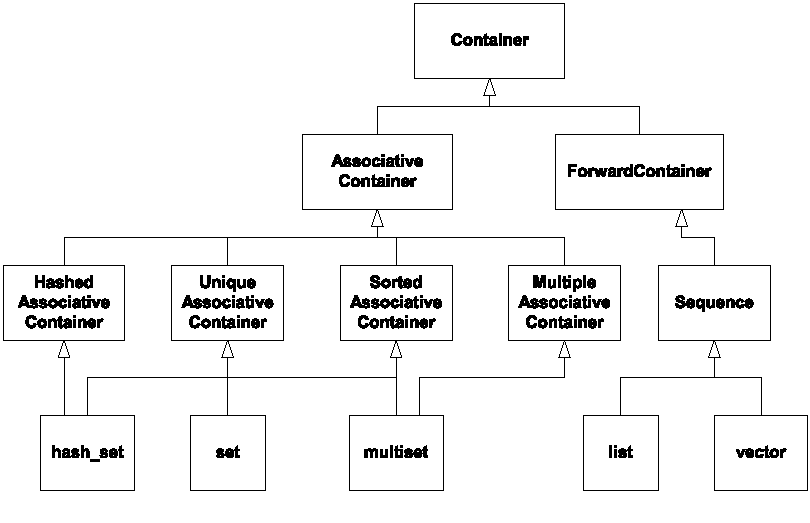
\includegraphics{STL/Containers.pdf}
    \end{center}  
    \caption{The class/interface hierarchy leading to the STL collections
             (sets, list and vector).
             \label{figContainers}} 
  \end{figure}
%\end{latexonly}  

%\begin{htmlonly}
%  \begin{rawhtml}
%    <center>
%      <img src="STL/Containers.gif">
%    </center>
%    <br>
%    <center>
%        The class/interface hierarchy leading to the STL collections
%             (sets, list and vector).
%    </center>
%  \end{rawhtml}  
%  \begin{figure}\label{figContainers}\end{figure}
%  \vspace{5mm}
%\end{htmlonly}  

All these collection classes are heavily parametrized. We shall discuss
a few of them below.

%\begin{latexonly}
  \begin{figure}[htb]
    \begin{center}  
      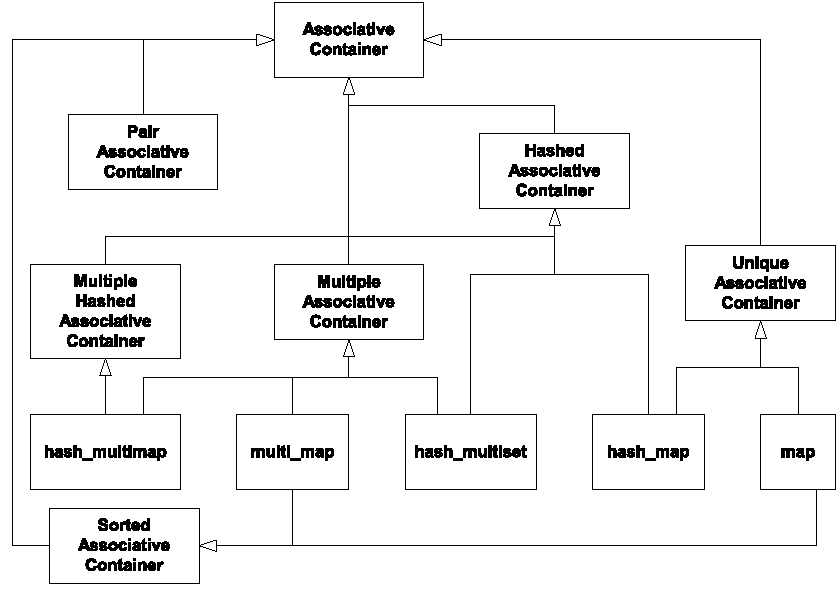
\includegraphics{STL/Maps.pdf}
    \end{center}  
    \caption{The class/interface hierarchy leading to the STL maps.
             \label{figMaps}} 
  \end{figure}
%\end{latexonly}  

%\begin{htmlonly}
%  \begin{rawhtml}
%    <center>
%      <img src="STL/Maps.gif">
%    </center>
%    <br>
%    <center>
%        The class/interface hierarchy leading to the STL maps.
%    </center>
%  \end{rawhtml}  
%  \begin{figure}\label{figMaps}\end{figure}
%  \vspace{5mm}
%\end{htmlonly}  

%----------------------------------------------------------------------

\subsection{The vector container type}

The vector template class supplied by the STL is not really a true vector
in the mathematical sense but a automatically resizing array structure.

It takes one compulsory template argument, the data type, and one optional 
template arguments, an allocator which provides a facility to assign
your own low-level mechanism for memory allocation and de-allocation.

\noindent{\small \begin{verbatim}
template <class T, class Alloc> vector
\end{verbatim}}

In nearly all practical cases the default allocator is used and the second
template argument is ommited. This to create an empty vector of floating 
point numbers on the stack you could write the following statement:

\noindent{\small \begin{verbatim}
vector<double> vec1;
\end{verbatim}}

If you want to specify an initial size of 20 elements you could write the 
following statement:

\noindent{\small \begin{verbatim}
vector<double> vec2(20);
\end{verbatim}}

%---------------------------------------------------------

\subsection{An example program using a vector}

\noindent{\small \input{STL/Programs/TestVector.cpp}}


%---------------------------------------------------------

\subsection{An example program using a set and a map}

\noindent{\small \input{STL/Programs/TestMap.cpp}}
